% THIS DOCUMENT IS FOLLOWS THE VOLERE TEMPLATE BY Suzanne Robertson and James Robertson
% ONLY THE SECTION HEADINGS ARE PROVIDED
%
% Initial draft from https://github.com/Dieblich/volere
%
% Risks are removed because they are covered by the Hazard Analysis
\documentclass[12pt]{article}

\usepackage{booktabs}
\usepackage{xltabular}
\usepackage{hyperref}
\usepackage{graphicx}
\usepackage{multirow}
\hypersetup{
    bookmarks=true,         % show bookmarks bar?
      colorlinks=true,      % false: boxed links; true: colored links
    linkcolor=red,          % color of internal links (change box color with linkbordercolor)
    citecolor=green,        % color of links to bibliography
    filecolor=magenta,      % color of file links
    urlcolor=cyan           % color of external links
}

\newcommand{\lips}{\textit{Insert your content here.}}

%% Comments

\usepackage{color}

\newif\ifcomments\commentstrue %displays comments
%\newif\ifcomments\commentsfalse %so that comments do not display

\ifcomments
\newcommand{\authornote}[3]{\textcolor{#1}{[#3 ---#2]}}
\newcommand{\todo}[1]{\textcolor{red}{[TODO: #1]}}
\else
\newcommand{\authornote}[3]{}
\newcommand{\todo}[1]{}
\fi

\newcommand{\wss}[1]{\authornote{blue}{SS}{#1}} 
\newcommand{\plt}[1]{\authornote{magenta}{TPLT}{#1}} %For explanation of the template
\newcommand{\an}[1]{\authornote{cyan}{Author}{#1}}

%% Common Parts

\newcommand{\progname}{ProgName} % PUT YOUR PROGRAM NAME HERE
\newcommand{\authname}{Team \#, Team Name
\\ Student 1 name
\\ Student 2 name
\\ Student 3 name
\\ Student 4 name} % AUTHOR NAMES                  

\usepackage{hyperref}
    \hypersetup{colorlinks=true, linkcolor=blue, citecolor=blue, filecolor=blue,
                urlcolor=blue, unicode=false}
    \urlstyle{same}
                                


\begin{document}

\title{Software Requirements Specification for \progname: Tangled Program Graphs} 
\author{\authname}
\date{\today}
	
\maketitle

~\newpage

\pagenumbering{roman}

\tableofcontents

~\newpage

\section*{Revision History}

\begin{tabularx}{\textwidth}{p{3cm}p{2cm}X}
\toprule {\textbf{Date}} & {\textbf{Version}} & {\textbf{Notes}}\\
\midrule
Oct. 8, 2024 & 1.0 & Intial draft of SRS document.\\
% Date 2 & 1.1 & Notes\\
\bottomrule
\end{tabularx}

~\\

~\newpage
\section{Purpose of the Project}
\subsection{User Business}
The Tangled Program Graphs (TPG) framework is an alternative approach to reinforcement learning (RL) that leverages evolution-based techniques instead of the widely used deep neural networks (DNN). In traditional RL, agents learn through trial and error by generating actions and receiving rewards. The DNN approach requires extensive computational resources, often involving thousands of GPUs, which can be expensive and inefficient. In contrast, TPG aims to provide a more cost-effective and resource-efficient solution, with the long-term goal of embedding this evolution-based learning directly into hardware, reducing dependency on large-scale computational infrastructure.

Currently, TPG has been tested primarily in fully observable, stationary mini-game environments, which are not representative of the dynamic and partially observable nature of real-world scenarios. This limitation presents a challenge, as the real-world problems TPG is meant to address are much more complex and constantly changing. To safely and effectively evolve TPG's capabilities, it is crucial to test the framework in advanced simulation environments, like MuJoCo, which can better mimic real-life dynamics in a controlled and risk-free manner.

Additionally, TPG's codebase has been developed by graduate students primarily focused on research output, often neglecting the software engineering practices necessary for creating a robust and maintainable open-source framework. Without standardized practices such as unit testing, continuous integration/continuous deployment (CI/CD), and architectural guidelines, TPG's long-term goal of becoming a widely adopted, open-source framework could be hindered. This project seeks to address these gaps, ensuring that TPG can scale, evolve, and attract contributions from other researchers and reinforcement learning enthusiasts in a standardized and efficient manner.
\subsection{Goals of the Project}

\begin{enumerate}
  \item \textbf{Enabling Software Engineering Standards}: We aim to create a seamless and standardized process for all contributors to the Tangled Program Graphs (TPG) framework. This includes simplifying the onboarding process, establishing clear contribution guidelines, and building a robust, scalable architecture that is open for extension but closed for modification. By doing so, we ensure that future development is both collaborative and sustainable, allowing for a consistent quality of contributions while maintaining the integrity of the core framework.
  \item \textbf{Physics Engine Integration}: We also seek to enhance TPG's ability to handle more complex, real-world-like scenarios. This will be achieved by integrating TPG with the MuJoCo physics engine, which allows for experimentation in dynamic and partially observable environments. By expanding the testing environments, we can evolve TPG's capabilities beyond its current limits, ensuring it is better suited for real-world applications.
\end{enumerate}

\section{Stakeholders}
\subsection{Client}
% \lips
\begin{itemize}
  \item \textbf{Description:} Dr. Stephen Kelly and his research team. They are responsible for the development and overseeing changes made to the TPG framework.
    \begin{itemize}
      \item \textbf{Role:} Main decision-makers on the scope and direction of the project. They will provide feedback on the project and approve the final implementation.
    \end{itemize}

  \end{itemize}





\subsection{Customer}
\textbf{N/A}
\begin{itemize}
\item \textbf{Reasoning:} This project is not a commercial product made for an intended customer audience in mind, but an extension to an existing research project.
\end{itemize}


\subsection{Other Stakeholders}
\begin{itemize}

\item \textbf{Description:} External French research team (GEGELATI). They are an organization that is adopting the TPG algorithm for research purposes differing from Dr Kelly’s project.
\begin{itemize}
  \item \textbf{Role:} Access to a more robust and maintainable framework for testing RL algorithms in high-fidelity simulators like MuJoCo. They may also share findings that may be beneficial to Dr Kelly’s research as well.

\end{itemize}


\item \textbf{Description:}The broader reinforcement learning research community. This includes research organizations and teams working with evolutionary algorithms and genetic programming who may be interested in Dr. Kelly’s research.
\begin{itemize}
  \item \textbf{Role:} End-users who will benefit from the enhancements made to the TPG framework, especially in the form of improved documentation, testing, and real-world applicability. The framework may be utilized or referenced in other research and contribute to further development of the field.

\end{itemize}

\end{itemize}

\subsection{Hands-On Users of the Project}
\begin{itemize}
  \item \textbf{Description:}  Researchers and developers working directly on the TPG framework. This includes Ph.D. students and collaborators involved in testing and developing within the codebase.
    \begin{itemize}
      \item \textbf{Role:} Active users who will interact with the code, run experiments, and test integrations (e.g., with MuJoCo). They are responsible for ensuring that the system works as intended and fits the project's research goals.

    \end{itemize}

  \end{itemize}

\subsection{Personas}
\begin{itemize}
  \item \textbf{Researcher Persona:}   Dr Stephen Kelly is a postdoctoral researcher focusing on genetic programming in predictive control environments. He is interested in how emergent forms of memory and hierarchy allow digital evolution to build programs in complex, multi-task environments, which he works on through his project -  the TPG framework. His goal is to evaluate and test TPG in complex environments, such as MuJoCo, to further his research in the field of RL. Dr Kelly is driven by the prospect of publishing impactful research and contributing to the RL community. However, he finds the lack of user-friendly documentation in TPG frustrating, as it makes setting up experiments and testing difficult. Despite this, Alex is committed to using TPG to demonstrate how genetic programming can outperform or complement traditional RL methods. He regularly uses technologies such as C++ for his work, and utilizes Gitlab for version control. He also aims to keep his project as an open source framework to allow others to benefit from his research.

  \item \textbf{Developer Persona:} Oliver is a software developer with a background in C++ and knowledge in the fundamentals of software engineering best practices. Currently, Jamie is working with Dr. Kelly’s research group to improve the TPG framework. His primary focus is to introduce modern software engineering principles, such as continuous integration, automated testing, and comprehensive documentation, to enhance the maintainability and scalability of TPG. Jamie is highly motivated to refactor the TPG codebase to make it more user-friendly for other researchers and contributors. However, he will have to balance the challenge of modernizing the codebase without disrupting the existing functionality or performance of TPG, especially without the full context of the system when he starts to work on it. Additionally, he will also be contributing to work on extending TPG to be integrated with Mujoco, an advanced physics simulator. He will be doing research on the best ways to create an integration between the two systems.

  \end{itemize}
\subsection{Priorities Assigned to Users}

\textbf{N/A}

\subsection{User Participation}
\begin{itemize}
  \item Hands-on users (researchers and developers) will be actively involved throughout the project lifecycle, providing feedback on codebase refactoring, testing, CI development and the MuJoCo integration.


  \item Frequent discussions with the Dr. Kelly and the research team during the development process, with periodic reviews at project milestones.

  \item The reinforcement learning community or other research organizations may provide indirect feedback post-development through research papers, informal discussion, and open-source contributions


  \end{itemize}
\subsection{Maintenance Users and Service Technicians}
The future maintainers of the TPG framework will likely be within Dr. Kelly’s research group or external contributors from the open-source community, will handle ongoing updates, bug fixes, and enhancements. User documentation will be provided to help improve the maintainability of the project.


\section{Mandated Constraints}
\subsection{Solution Constraints}
The solution must strictly adhere to modern software engineering best practices, including comprehensive documentation, robust testing, and the implementation of continuous integration and continuous deployment (CI/CD) pipelines. The implementation must be in C++ to maintain compatibility with the existing Tangled Program Graphs (TPG) codebase. The system must integrate seamlessly with MuJoCo, a physics engine developed by Google DeepMind, to enable testing in dynamic and partially observable environments. All code contributions must comply with open-source licensing agreements and standards to facilitate community collaboration. Additionally, the solution should minimize computational resource requirements to support deployment on embedded systems with limited processing capabilities.

\subsection{Implementation Environment of the Current System}
The current TPG framework is implemented in C++. MuJoCo is originally written in C, and its core API is in C, so interacting with C++ is a good option. Development will occur in a UNIX-like environment with as much standardization as possible. Virtualization environments such as Docker, VSCode Dev Containers, WSL, and VMs will be considered based on the ease of environment standardization across the team. OpenGL will be used to display the RL simulation, so display compatibility with the virtualization environments will need to be considered.

\subsection{Partner or Collaborative Applications}
\lips
\subsection{Off-the-Shelf Software}
\lips
\subsection{Anticipated Workplace Environment}
\lips
\subsection{Schedule Constraints}
\lips
\subsection{Budget Constraints}
\lips
\subsection{Enterprise Constraints}
\lips

\section{Naming Conventions and Terminology}
\subsection{Glossary of All Terms, Including Acronyms, Used by Stakeholders
involved in the Project}
% \lips
\begin{description}
  \item [Agent]\label{def:agent} An autonomous intelligence system performed to do specific tasks without human assistance.
  \item [Environment]\label{def:environment} This is referred to the external system that the agent interacts with. The environment can provide information such as the current state and reward, and the agent can provide the environment with its action.
  \item [Tangled Program Graphs (TPG)]\label{def:tpg} A framework currently being developed under Dr. Stephen Kelly that will help modular programs apply genetic programming principles to embedded systems.
  \item [Deep Neural Networks (DNNs)]\label{def:dnn} A machine learning technique that trains an agent to complete difficult tasks that would be difficult to do using conventional programming.
  \item [Genetic Programming]\label{def:genetic_programming} A technique used to evolve programs, that first start a population of “unfit” agents. Through RL, agents are destroyed, kept, and mutated to evolve into a more suitable population. This is continued until the population reaches its desired fit.
  \item [Reinforcement Learning (RL)]\label{def:rl} A machine learning technique that utilizes a reward-and-punishment system towards agents, providing a reward for a correctly done task and a punishment for incorrectly done tasks.
  \item [Multi-Task Reinforcement Learning (Multi-Task RL)]\label{def:mulittask_rl} A type of reinforcement learning in which agents are learning multiple tasks at the same time.
  \item [Policy]\label{def:policy} A strategy that a particular agent uses to complete a specific task. This is also known as agent behaviour. 
  \item [MuJoCo]\label{def:mujoco} A free and open-source physics engine created by Google DeepMind that assists in facilitating research and development in areas such as robotics.
  \item [Phylogenetic Learning]\label{def:phylogenetic_learning} Also known as Policy Search, this is a class of reinforcement learning in which agent-environment interactions are episodic. The policy becomes updated as a whole following the final episode outcome.
  \item [Temporal Credit Assignment Problem]\label{def:temporal_credit} Actions with neutral or negative rewards may still contribute to a successful outcome.
  \item [Stationary Environments]\label{def:stationary_env} The transition function does not change over time.
  \item [Non-Stationary Environments]\label{def:nonstationary_env} Transition function changes over time. e.g. video games get harder the longer you play (physics of the world change)
  \item [Fully-Observable Environment]\label{fully_obs_env} The state contains all information required to make action decisions, e.g. Chess.
  \item [Partially-Observable Environment]\label{partial_obs_env} The state provides partial world-view, e.g. first-person perspective video games.
\end{description}

\section{Relevant Facts And Assumptions}
\subsection{Relevant Facts}
The Tangled Program Graphs (TPG) framework is currently implemented in C++ and is utilized for genetic programming in reinforcement learning (RL) environments. The existing codebase lacks comprehensive documentation, testing suites, and continuous integration/continuous deployment (CI/CD) pipelines, which hinders its usability and maintainability. Additionally, the integration of MuJoCo, a physics engine developed by Google DeepMind, is intended to enhance the TPG framework by enabling testing in dynamic and partially observable environments.

\subsection{Business Rules}
All code contributions must comply with open-source licensing agreements, such as the MIT license, to ensure that the framework remains accessible to researchers and developers. Secondly, any modifications to the codebase must be accompanied by comprehensive documentation and testing to maintain high standards of quality and usability, meeting the requirements of rigorous scientific research. Additionally, the project must implement a continuous integration/continuous deployment (CI/CD) pipeline to automate testing and deployment processes, ensuring that all changes are validated before integration into the main codebase.

\subsection{Assumptions}
It is assumed that all team members possess a working knowledge of C++ and are familiar with software engineering best practices. Furthermore, it is expected that the necessary computing resources and development tools will be available and accessible to the team throughout the project duration. The integration of MuJoCo into the TPG framework is presumed to be feasible without encountering insurmountable licensing or technical impediments. Additionally, it is anticipated that external contributors from Dr. Kelly's research group may become involved after the development phase, necessitating clear guidelines and documentation for collaboration.

\section{The Scope of the Work}
\subsection{The Current Situation}

For the scope of this capstone, there are two main areas of focus: Software Engineering practices and physics engine integration. Both of these have current states which will be improved upon over the course of this project.

\subsubsection{Software Engineering Practices}
The TPG (Tangled Program Graph) project is currently managed with basic software engineering practices. The codebase is hosted on GitLab, and Dr. Kelly’s research group uses Git branches to separate and manage their work. This current setup does allow for parallel work and multiple contributors.
However, several key practices are missing:
\begin{itemize}
  \item Unit Testing: There are no unit tests in place. This absence means that code changes are not systematically validated, increasing the risk of introducing bugs and regressions.
  \item Continuous Integration/Continuous Deployment (CI/CD): The project lacks automated pipelines for building, testing, and deploying code. Without CI/CD, integrating changes can be time-consuming and error-prone.
  \item Pull Request Templates and Standards: There are no standardized templates or guidelines for pull requests, leading to inconsistencies in code reviews and collaboration.
  \item Open Source License: The project has not yet adopted an open-source license, which can deter external contributions and limit the software's usage.
  \item Issue Management: There is no formal system for tracking bugs, feature requests, or tasks, making project management less efficient. 
\end{itemize}
The current structure of the TPG codebase may not be optimized for use as an open-source library. Current researchers need to run shell scripts as the entry point, which can be a barrier to entry for those unfamiliar with the system. Additionally, MacOS with ARM based chips may have extra difficulty in onboarding to this project due to the many dependency conflicts in this current state. This approach limits accessibility and may discourage potential users and contributors. More research into code structure and analysis of how other open source libraries allow for their frameworks to be integrated into open source contributor workflows should be studied.

\subsubsection{Physics Engine Integration}

The TPG framework has been validated using OpenAI Gym's classic control problems such as CartPole, Acrobot, and Pendulum. These environments are stationary, meaning their transition functions (the rules determining the next state given a current state and action) do not change over time.
In contrast, real-world environments are typically non-stationary. Their transition functions can evolve due to external factors, requiring agents to adapt continuously. Currently, the TPG framework needs to evolve and be adapted to more dynamic environments.

\subsection{The Context of the Work}

\subsubsection{Software Engineering Practices}

\begin{figure}[h!]
  \begin{center}
   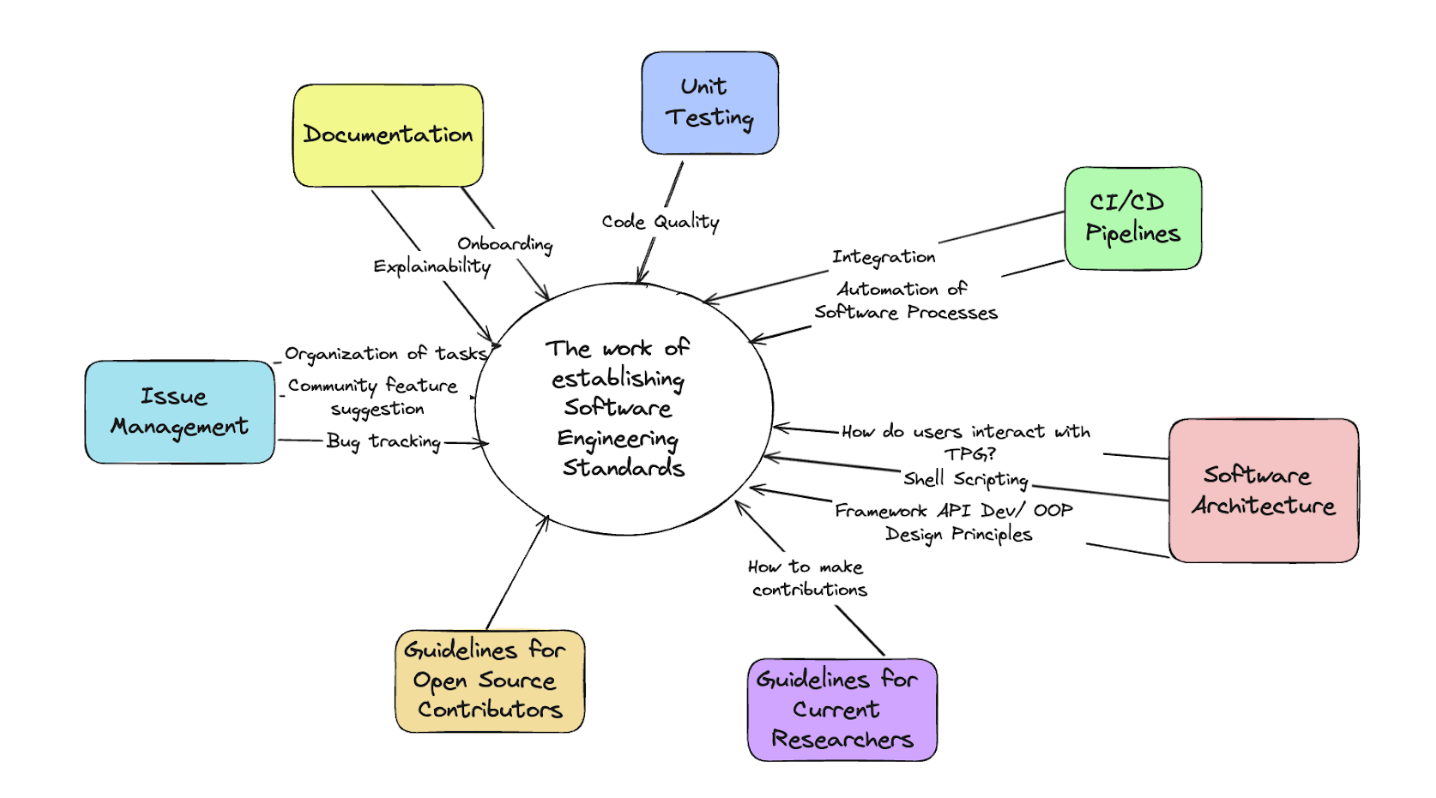
\includegraphics[scale=0.6]{SystemContext.png}
  \caption{System Context}
  \label{Fig_SystemContext} 
  \end{center}
\end{figure}

\begin{itemize}
  \item Unit Testing: Focused on improving code quality, unit tests ensure that individual pieces of the codebase work as expected.
  \item CI/CD Pipelines: The integration and automation of software processes, such as building and testing, will allow for continuous integration and deployment of changes, ensuring the project remains robust as it scales.
  \item Software Architecture: This examines how users interact with TPG, the use of shell scripting, and how the framework is structured using API development and object-oriented programming (OOP) principles. It emphasizes improving design principles for a better developer and user experience.
  \item Documentation: This is critical for onboarding new developers, ensuring explainability, and providing clear, thorough project documentation.
  \item Issue Management: Introducing a formal system to track bugs, feature requests, and community suggestions will help organize tasks and streamline project development.
  \item Guidelines for Open Source Contributors: Establishing clear guidelines will provide a roadmap for external contributors to participate in the project, increasing collaboration and contributions.
  \item Guidelines for Current Researchers: This component covers how researchers and developers within the project can contribute effectively, ensuring consistency and alignment with the project's goals.
\end{itemize}

\subsubsection{Physics Engine Integration}
\begin{figure}[hbt!]
  \begin{center}
   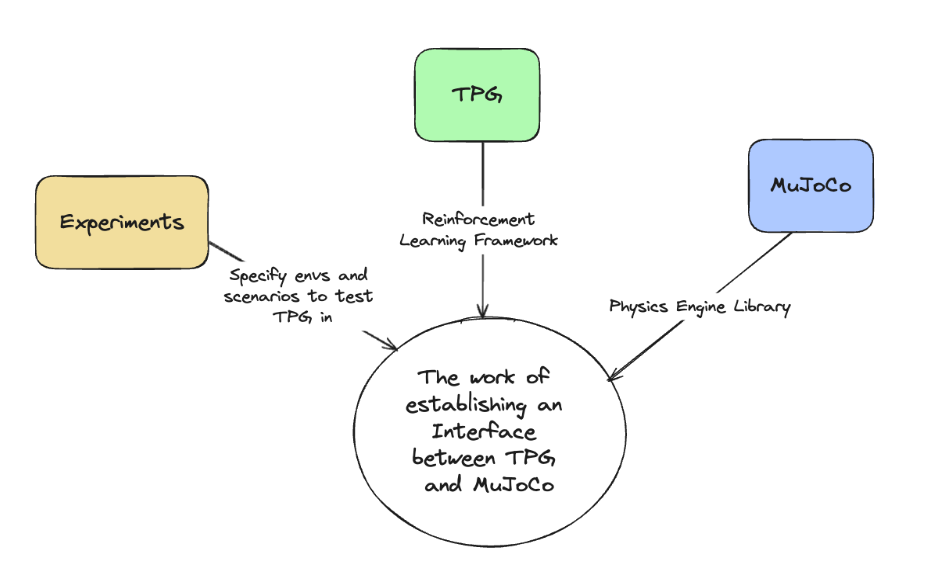
\includegraphics[scale=0.5]{PhysicsEngineContext.png}
  \caption{System Context}
  \label{Fig_PhysicsEngineContext} 
  \end{center}
\end{figure}

\begin{itemize}
  \item TPG (Tangled Program Graphs): TPG is a reinforcement learning framework. In this context, its role is to act as the core system that will be tested and integrated with dynamic environments. Establishing the interface between TPG and MuJoCo will allow the TPG framework to be tested in physically realistic simulations.
  \item MuJoCo (Multi-Joint dynamics with Contact): MuJoCo is a high-performance physics engine used for modeling and simulating dynamic systems. In this diagram, it represents the external library that provides the physics-based environments required for testing TPG. The interface with TPG will enable the reinforcement learning agents created using TPG to interact with complex, real-world-like physics simulations provided by MuJoCo.
  \item Experiments: Experiments define the environments and scenarios where TPG will be tested. This component represents the experimental setups that specify the parameters for evaluating TPG’s performance in various MuJoCo-based scenarios. These experiments are critical for determining how well TPG adapts to different physics-based tasks, environments, and scenarios.
\end{itemize}

\subsection{Work Partitioning}

\begin{xltabular}{\textwidth}{   
  | >{\raggedright\arraybackslash}X 
  | >{\raggedright\arraybackslash}X 
  | >{\raggedright\arraybackslash}X 
  | >{\raggedright\arraybackslash}X | }
  \caption{Work Partitioning Table} \\
  
  \hline \multicolumn{1}{|c|}{\textbf{Event Name}} & \multicolumn{1}{c|}{\textbf{Inputs}} & \multicolumn{1}{c|}{\textbf{Outputs}} & \multicolumn{1}{c|}{\textbf{Summary}} \\ \hline 
  \endfirsthead
  
  \multicolumn{4}{c}%
  {\tablename\ \thetable{} -- continued from previous page} \\
  \hline \multicolumn{1}{|c|}{\textbf{Event Name}} & \multicolumn{1}{c|}{\textbf{Inputs}} & \multicolumn{1}{c|}{\textbf{Outputs}} & \multicolumn{1}{c|}{\textbf{Summary}} \\ \hline 
  \endhead
  
  \hline \multicolumn{4}{|r|}{{Continued on next page}} \\ \hline
  \endfoot
  \hline
\endlastfoot
\hline
Contributor wants to merge code changes they made & New changes (code that was modified in a PR) & New code is successfully integrated with the main code & CI - Continuous Integration practices into the repo, ensuring all devs can make changes in a seamless manner and be up to date while concurrent work is occuring \\
\hline
Contributor wants to evaluate the code they wrote & New code blocks that are written by a contributor & Test functions are created to evaluate new code & Automated tests are generated for new code blocks that are written ensuring code robustness \\
\hline
Contributor wants to onboard and use TPG & N/A & Contributor is able to run the framework & Seamless onboarding experience that allows a new contributor/user to get up and running \\
\hline
Contributor wants to perform an experiment to test the TPG framework in MuJoCo & TPG, MuJoCo & Functioning simulation of an experiment integrated with a physics engine & New experiments to be conducted in more realistic scenarios evolving the development of this reinforcement learning framework \\
\hline
Contributor wants to get visual results of from test data & TPG, MuJoCo & Graphs of the recent experiment & Evaluation of the experiment is crucial to improving the framework and allowing it to become good at multi task reinforcement learning tasks \\

\end{xltabular}

\section{Business Data Model and Data Dictionary}
\subsection{Business Data Model}
\subsubsection{Software Engineering Practices}

\begin{figure}[ht!]
  \begin{center}
   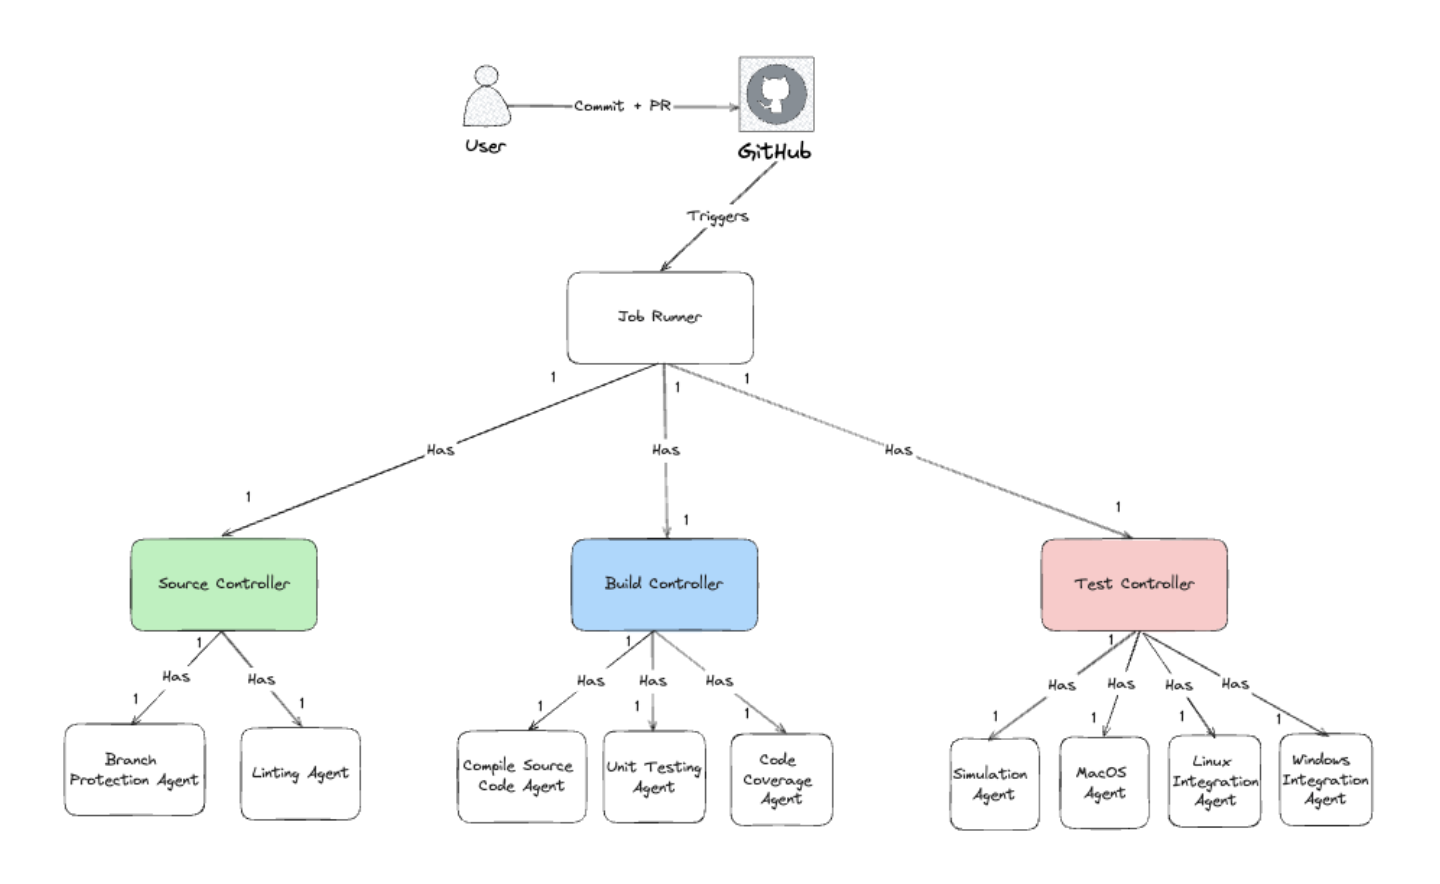
\includegraphics[scale=0.5]{DataModel.png}
  \caption{Data Model}
  \label{Fig_DataModel} 
  \end{center}
\end{figure}

\clearpage

Figure 3 illustrates a UML data model of a traditional CI/CD pipeline implemented using GitHub Actions. The architecture follows a master-slave design pattern, where the pipeline steps are defined in a YAML configuration file. For each step in the pipeline, a Controller (master) class orchestrates the process by delegating tasks to Agents (slaves) that handle specific actions. This design is commonly used in CI/CD pipelines because it reflects the sequential nature of the CI/CD process—each step must wait for the previous one to complete before proceeding.

\subsubsection{Physics Engine Integration}

\begin{figure}[ht!]
  \begin{center}
   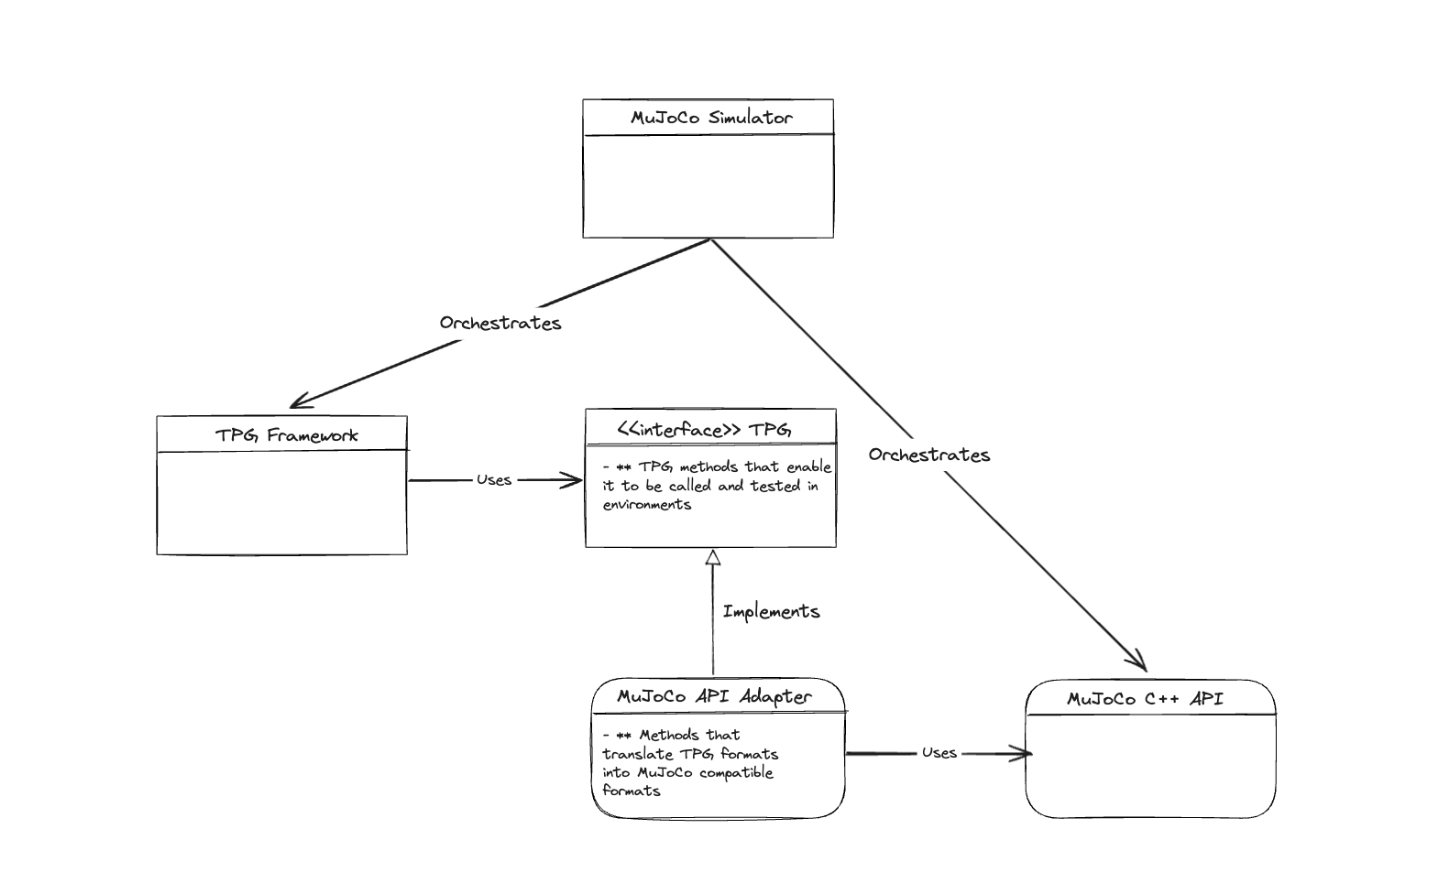
\includegraphics[scale=0.5]{ClassModel.png}
  \caption{Physics Engine Class Diagram}
  \label{Fig_ClassModel} 
  \end{center}
\end{figure}

Figure 4 presents a simplified UML data model of the interface being developed to integrate the TPG framework with MuJoCo. The primary objective is to adapt how the TPG framework handles state changes into a format that MuJoCo can interpret. To achieve this, we are utilizing the Adapter design pattern to translate incompatible formats and ensure compatibility between the two systems.

\subsection{Data Dictionary}

\begin{xltabular}{\textwidth}{   
  | >{\raggedright\arraybackslash}X 
  | >{\raggedright\arraybackslash}X 
  | >{\raggedright\arraybackslash}X | }
  \caption{Data Dictionary Table} \\
  
  \hline \multicolumn{1}{|c|}{\textbf{Name}} & \multicolumn{1}{c|}{\textbf{Content}} & \multicolumn{1}{c|}{\textbf{Type}} \\ \hline 
  \endfirsthead
  
  \multicolumn{3}{c}%
  {\tablename\ \thetable{} -- continued from previous page} \\
  \hline \multicolumn{1}{|c|}{\textbf{Name}} & \multicolumn{1}{c|}{\textbf{Content}} & \multicolumn{1}{c|}{\textbf{Type}} \\ \hline 
  \endhead
  
  \hline \multicolumn{3}{|r|}{{Continued on next page}} \\ \hline
  \endfoot
  \hline
\endlastfoot
\hline
Job Runner & Orchestrates all the jobs for the GitHub Actions CI/CD Pipeline & Class \\
\hline
Source Controller & Responsible for orchestrating Branch Protection rules and Linting during the Source stage of the CI/CD Pipeline & Class \\
\hline
Branch Protection Agent & Responsible for enabling branch protection on the repo to prevent accidental integrations on the main branch & Class \\
\hline
Linting Agent & Static analysis on the code and cleans it up & Class \\
\hline
Build Controller & Responsible for orchestrating the Build stage of the CI/CD Pipeline & Class \\
\hline
Compile Source Code Agent & Compiles the code to prepare it for validation & Class \\
\hline
Unit Testing Agent & Runs through all the unit tests in an automated fashion & Class \\
\hline
Code Coverage Agent & Static analyzes the coverage from the unit tests, usually needs to be above 85\% & Class \\
\hline
Test Controller & Responsible for orchestrating the Test stage of the CI/CD Pipeline & Class \\
\hline
MacOS, Linux, Windows Agents & Containers for each OS to test the integration of the framework in each environment (industry standard) & Class \\
\hline
Simulation Agent & Responsible for integration testing to ensure the new changes are robust and don’t break & Class \\

\end{xltabular}

\section{The Scope of the Product}
\subsection{Product Boundary}

\begin{xltabular}{\textwidth}{   
  | >{\raggedright\arraybackslash}X 
  | >{\raggedright\arraybackslash}X | }
  \caption{Product Boundary} \\
  
  \hline \multicolumn{1}{|c|}{\textbf{In Scope}} & \multicolumn{1}{c|}{\textbf{Out of Scope}} \\ \hline 
  \endfirsthead
  
  \multicolumn{2}{c}%
  {\tablename\ \thetable{} -- continued from previous page} \\
  \hline \multicolumn{1}{|c|}{\textbf{In Scope}} & \multicolumn{1}{c|}{\textbf{Out of Scope}} \\ \hline 
  \endhead
  
  \hline \multicolumn{2}{|r|}{{Continued on next page}} \\ \hline
  \endfoot
  \hline
\endlastfoot
\hline
CI/CD Pipeline: Software Engineering practices need to be integrated into the code base & Ongoing research experiments with TPG: Since Dr. Kelly and his grad students are still developing TPG, the scope of our capstone won’t encompass current efforts \\
\hline
Interface between MuJoCo + TPG: Development of the interface that enables testing and evaluation of TPG in a physics engine must be established & \\
\hline
Code refactoring: Reorganizing code structure to make it suitable as a C API to allow open source contributions/seamless integrations into other projects & \\

\end{xltabular}

\subsection{Product Use Case Table}

\begin{xltabular}{\textwidth}{   
  | >{\raggedright\arraybackslash}X 
  | >{\raggedright\arraybackslash}X | }
  \caption{Product Boundary} \\
  
  \hline \multicolumn{1}{|c|}{\textbf{User}} & \multicolumn{1}{c|}{\textbf{Use Case}} \\ \hline 
  \endfirsthead
  
  \multicolumn{2}{c}%
  {\tablename\ \thetable{} -- continued from previous page} \\
  \hline \multicolumn{1}{|c|}{\textbf{User}} & \multicolumn{1}{c|}{\textbf{Use Case}} \\ \hline 
  \endhead
  
  \hline \multicolumn{2}{|r|}{{Continued on next page}} \\ \hline
  \endfoot
  \hline
\endlastfoot
\hline

\multirow{2}{0.5\textwidth}{Researchers in Dr. Kelly’s research group} & - When researcher make changes to the code base, they are able to validate their logic through unit testing, integration testing in the CI/CD pipeline \\
& - Perform experimentations using TPG in a physics engine, to further improve the reinforcement learning framework \\
& - Access the code not by only using shell scripts, but through the C API \\
& - Share how the integration is done in an Open Source manner to allow other community members to access the code \\
& - Issue management to organize who is working on what currently \\

\multirow{2}{0.5\textwidth}{Open Source Contributors} & - Access and embed the TPG framework into their own applications \\
& - Make changes to the TPG framework in an automated manner \\
& - Suggest changes to the framework in an standardized way \\

\end{xltabular}

\subsection{System Boundaries}
\subsubsection{GitHub Actions Pipeline}

\begin{figure}[ht!]
  \begin{center}
   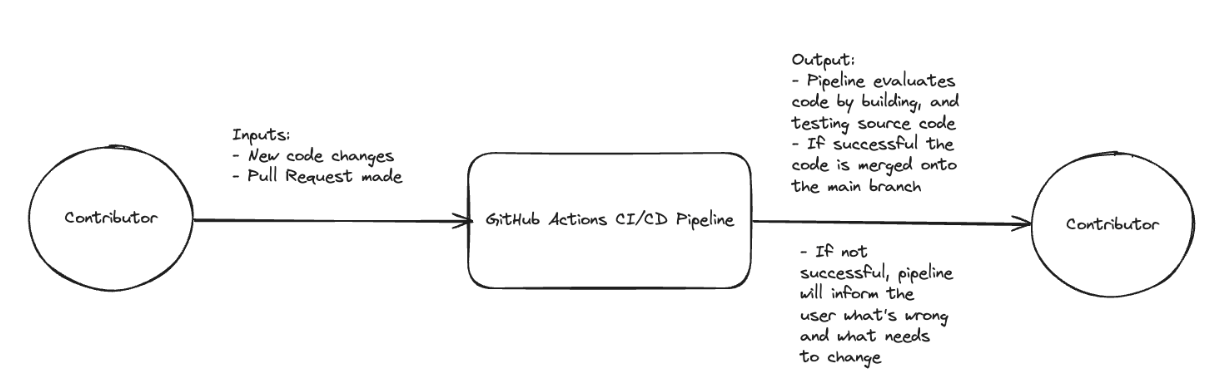
\includegraphics[scale=0.5]{GitHubActionsSystem.png}
  \caption{GitHub Actions Pipeline System Boundary}
  \label{Fig_GitHubActions} 
  \end{center}
\end{figure}

\subsubsection{Physics Engine Integration}

\begin{figure}[ht!]
  \begin{center}
   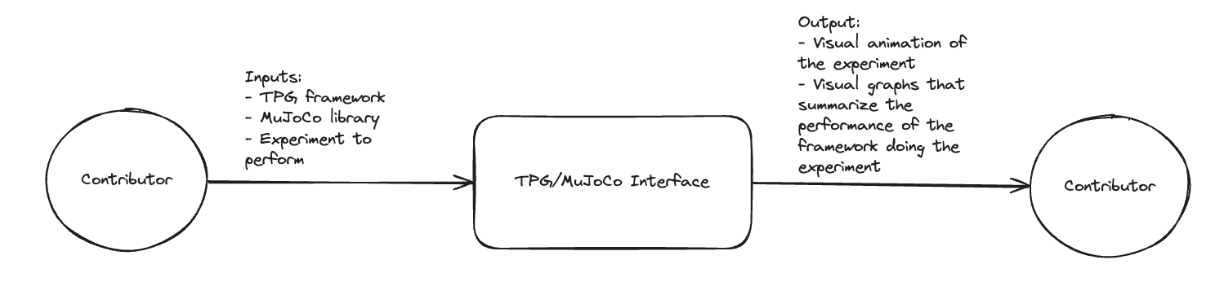
\includegraphics[scale=0.5]{PhysicsIntegration.png}
  \caption{MuJoCo Physics Integration}
  \label{Fig_MuJoCo} 
  \end{center}
\end{figure}

\subsection{Formalized Math and Application Flow}
\subsubsection{Software Engineering Practices}

Definitions: Let C be the set of all code changes, T be the set of all tests, S be the set of all test successes, E be the set of all test failures

Functions:
\begin{enumerate}
  \item \begin{math}
    Success: C \cap T \rightarrow S
  \end{math}
  \item \begin{math}
    Failure: C \cap T \rightarrow E
  \end{math}
\end{enumerate}

\subsubsection{Physics Engine Integration}

Definitions: Let T represent the TPG framework, M represent the MuJoCo framework, E represent the experiment

Relation:
\begin{enumerate}
  \item \begin{math}
    R \subseteq E \cup (T \cap M)
  \end{math}
\end{enumerate}

\section{Functional Requirements}
\subsection{Functional Requirements}
% \lips
\begin{itemize}
\item \textbf{FR-1:} The system shall have an interface that is compatible with \hyperref[def:mujoco]{MujoCo}.
  \begin{itemize}
    \item \textbf{Rationale:} This is a requirement brought on by the stakeholders to have an interface that integrates \hyperref[def:tpg]{TPG} with the \hyperref[def:mujoco]{MuJoCo} environment.
  \end{itemize}
\item \textbf{FR-2:} The system shall be able to visualize an experiment running from test data.
  \begin{itemize}
    \item \textbf{Rationale:} Visualizing the experiment from test data will allow for verification of the simulator and interface compatibility.
  \end{itemize}
\item \textbf{FR-3:} The system shall have an integrated CI/CD pipeline.
  \begin{itemize}
    \item \textbf{Rationale:} To have a good workflow environment for the development of the project, a CI/CD pipeline is a beneficial way to do so.
  \end{itemize}
\item \textbf{FR-4:} The system shall automatically run test cases once a new code change has been detected in the main branch.
  \begin{itemize}
    \item \textbf{Rationale:} This is to ensure that all test cases pass when a new code update has been implemented and breakage of code or functionality is not all introduced.
  \end{itemize}
\item \textbf{FR-5:} The system shall be automatically compiled and built once all automated test cases have passed.
  \begin{itemize}
    \item \textbf{Rationale:} Once all test cases have passed, the system can safely ensure that the update can be implemented into the code.
  \end{itemize}
\item \textbf{FR-6:} The system shall adhere to standard software engineering code practices.
\begin{itemize}
  \item \textbf{Rationale:} This is to allow for easy maintainability of the code. As this is a research project, the people working on the project will be constantly changing. Adhering to these practices minimizes development hassle.
\end{itemize}
\item \textbf{FR-7:} The system shall perform automatic code linting before building the project.
\begin{itemize}
  \item \textbf{Rationale:} Code linting will allow for universal and consistent formatting of code within the project. 
\end{itemize}
\item \textbf{FR-8:} The system shall be able to adapt to new experiments provided by the simulator without any downtime. 
  \begin{itemize}
    \item \textbf{Rationale:} This is important as the system should not be dependent on the experiments being simulated, rather the interface shall be able to adapt easily to newly introduced experiments. 
  \end{itemize}
\end{itemize}
\section{Look and Feel Requirements}

\subsection{Appearance Requirements}

\begin{itemize}
  \item \textbf{LFAR1:}  The codebase should follow clear and consistent formatting guidelines. This includes proper indentation, descriptive variable names, and potentially inline documentation to enhance readability for both new and experienced project developers.
      \begin{itemize}
        \item \textbf{Rationale:} A consistent code style and formatting increases the maintainability of the project and allows developers to easily understand and contribute to the project. 
      \end{itemize}
\end{itemize}


\subsection{Style Requirements}


\begin{itemize}
  \item \textbf{LFSR1:}  The style of the code, including naming conventions, commenting, and structure, should remain consistent across all modules of the TPG framework.

      \begin{itemize}
        \item \textbf{Rationale:} This consistency will ensure a cohesive development experience and make the project easier to maintain and expand in the future.
      \end{itemize}
\end{itemize}


\section{Usability and Humanity Requirements}
\subsection{Ease of Use Requirements}
\begin{itemize}
  \item \textbf{UH-E1:} The system shall have a clear and comprehensive documentation.
  \begin{itemize}
    \item \textbf{Rationale:} A consistent and comprehensive documentation on the CI/CD pipeline and agent-environment integration ensures ease of usage for all future users regardless of their technical level.
  \end{itemize}
  \item \textbf{UH-E2:} The system shall provide real-time, accurate logging of messages for every action.
  \begin{itemize}
    \item \textbf{Rationale:} Real-time, accurate logging of messages allows users to understand the outcome of their inputs instantaneously, reducing confusion, habilitating more opportunities for debugging and empowers users of their expectations.
  \end{itemize}
\end{itemize}


\subsection{Personalization and Internationalization Requirements}
\begin{itemize}
  \item \textbf{UH-PI1:} The system shall have the flexibility to adjust certain parameters when configuring MuJoCo.
  \begin{itemize}
    \item \textbf{Rationale:} Having the flexibility to change parameters provides users the opportunity to make the system fit to their specific needs and requirements.
  \end{itemize}
\end{itemize}

\subsection{Learning Requirements}
\begin{itemize}
  \item \textbf{UH-L1:} The system shall have tutorials available to the users.
  \begin{itemize}
    \item \textbf{Rationale:} Having tutorials, simulation examples and guides for the TPG framework and MuJoCo provides guidance to understand user interaction between the entire system and agent-environments.
  \end{itemize}
  \item \textbf{UH-L2:} The system shall ensure that relevant technical concepts and resources shall be accessible by users with ease.
  \begin{itemize}
    \item \textbf{Rationale:} Acknowledging that TPG builds up on several machine learning concepts, listing resources that will complement learning the framework can accelerate user onboarding.
  \end{itemize}
\end{itemize}

\subsection{Understandability and Politeness Requirements}
\begin{itemize}
  \item \textbf{UH-UP1:} The system shall accommodate symbols and words that are naturally understandable by all potential users.
  \begin{itemize}
    \item \textbf{Rationale:} In addition to having clear and concise message outputs, avoiding the use of slang, jargons or ambiguous terms minimizes confusion and learning curve for users. This includes using traditional symbols and words that the majority of the users are familiar with.
  \end{itemize}
  \item \textbf{UH-UP2:} The system shall not include offensive language in its logging.
  \begin{itemize}
    \item \textbf{Rationale:} Explicit, biased or unnaturally used language may harm any users. It is best for the framework to avoid using any words to ensure a healthy environment. The use of offensive languiage can create an unsafe relationship between the user and the system, compromising user trust.
  \end{itemize}
\end{itemize}

\subsection{Accessibility Requirements}
\begin{itemize}
  \item \textbf{UH-A1:} The system shall accommodate users with different kinds of disabilities.
  \begin{itemize}
    \item \textbf{Rationale:} Supporting features such as text-to-speech, and color blindness assistance systems can allow users with different kinds of disabilities to leverage TPG, fostering an inclusive environment.
  \end{itemize}
\end{itemize}

\section{Performance Requirements}
\begin{itemize}
\item \textbf{PR-SL:} The system shall execute without introducing significant computational overhead. The integration with MuJoCo must not degrade performance, and any additional computational costs should be minimized through optimization.
  \begin{itemize}
    \item \textbf{Rationale:} Ensures that processing times remain acceptable for real-time experimentation and testing.
  \end{itemize}

\item \textbf{PR-PA:} The system shall produce accurate and reliable results in simulations and experiments. All calculations must maintain high numerical precision to ensure the validity of results, especially when dealing with complex reinforcement learning tasks and physics simulations.
  \begin{itemize}
    \item \textbf{Rationale:} Ensures the validity of the reinforcement models being developed. Otherwise, inaccurate results can lead to incorrect conclusions and hinder the development of effective learning agents.
  \end{itemize}

\item \textbf{PR-RFT:} The system shall be robust against invalid inputs and unexpected environmental conditions. It must handle exceptions gracefully, recover from errors without data loss, and maintain operational stability under varying workloads and stress conditions.
  \begin{itemize}
    \item \textbf{Rationale:} In cases where the agent returns an action that is not defined by the environment, or the agent receives an out-of-bounds state, the system should be able to manage this gracefully.
  \end{itemize}

\item \textbf{PR-CR:} The system shall support scaling up to handle multiple simultaneous experiments or large-scale simulations without significant degradation in performance. Efficient resource management is essential to accommodate the demands of complex reinforcement learning tasks.
  \begin{itemize}
    \item \textbf{Rationale:} Efficient resource management is necessary to ensure that the system can accommodate the needs of diverse experiments without performance degradation.
  \end{itemize}

\item \textbf{PR-SE:} The system shall be designed for scalability, allowing for easy addition of new features, integration with other environments, and support for future research needs. The codebase should be modular and extensible, facilitating contributions from other researchers and developers.
  \begin{itemize}
    \item \textbf{Rationale:} The system should be designed for scalability to allow for future enhancements to the TPG algorithm and the addition of new environments within MuJoCo. A modular and extensible design will facilitate these updates and ensure that the framework remains relevant.
  \end{itemize}

\item \textbf{PR-RR:} The system shall maintain high reliability, with minimal downtime or failures during operation. Continuous integration and automated testing shall be employed to detect and address issues promptly, ensuring consistent performance over time.
  \begin{itemize}
    \item \textbf{Rationale:} High reliability is crucial for maintaining user trust and ensuring that experiments yield consistent results. Continuous integration and automated testing will help identify and address issues promptly, minimizing downtime and ensuring that the system operates smoothly over time.
  \end{itemize}
\end{itemize}

\section{Operational and Environmental Requirements}
\begin{itemize}
\item \textbf{OE-EPE:} The system will operate in typical computing laboratory environments, which may include personal computers or servers running UNIX-like operating systems. It should function effectively on standard hardware without the need for specialized equipment, supporting researchers and developers in academic settings.
  \begin{itemize}
    \item \textbf{Rationale:} Ensuring compatibility across different hardware allows for broader accessibility and usability among researchers and developers.
  \end{itemize}

\item \textbf{OE-RIA:} The system must interface seamlessly with existing environments, MuJoCo, and potentially other simulation environments. Compatibility requires adherence to their API specifications and proper handling of data exchange protocols. Any dependencies or libraries required for integration must be managed effectively.
  \begin{itemize}
    \item \textbf{Rationale:} Proper handling of data exchange protocols is essential for maintaining the integrity of experiments and ensuring that the TPG framework can be evaluated in diverse settings.
  \end{itemize}

\item \textbf{OE-RR:} The system shall be released under an appropriate open-source license (e.g., MIT license) to enable community collaboration. All releases must include comprehensive documentation, installation instructions, and user guides to assist researchers and developers in utilizing and contributing to the framework.
  \begin{itemize}
    \item \textbf{Rationale:} Releasing the system under an open-source license encourages collaboration and ensures accessibility for researchers and developers. Clear documentation and guides help users utilize and contribute effectively, fostering a collaborative environment for framework improvement.
  \end{itemize}

\item \textbf{OE-OSR:} Internal resources and mechanisms should be established to assist current and future members of the research group in utilizing and contributing to the TPG framework. This includes the GitHub repository and associated documentation such as this SRS report, troubleshooting resources, and history of issue tracking.
  \begin{itemize}
    \item \textbf{Rationale:} Improves efficiency of knowledge sharing and ensures continuity of the project as team members change over time.
  \end{itemize}
\end{itemize}

\section{Maintainability and Support Requirements}
\subsection{Maintenance Requirements}
% \lips

\begin{itemize}
  \item \textbf{MS-M1:} If a change is made to the finished software, it will take at most 15\% of the original development time, assuming the same development resources are available.
    \begin{itemize}
      \item \textbf{Rationale:} One of the goals of the project is to ensure a more efficient and smooth software structure. As such 15\% is an appropriate reduction in development time to verify the project’s efficiency. 
    \end{itemize}
  \item \textbf{MS-M2:} The software shall have detailed and organized code documentation.
  \begin{itemize}
    \item \textbf{Rationale:} Detailed and organized code documentation makes it easier for developers when it comes to traceability and verifiability. 
  \end{itemize}
  \item \textbf{MS-M3:} The software shall maintain regular updates, at least once a month, assuming a change regarding dependent frameworks or libraries has occurred. 
  \begin{itemize}
    \item \textbf{Rationale:} Maintaining regular updates is critical to ensure that the project is protected against any security or software bugs caused by the dependent frameworks. Ensuring updates at least once a month minimizes the risk of errors occurring. 
  \end{itemize}
\end{itemize}

\subsection{Supportability Requirements}
% \lips
\begin{itemize}
  \item \textbf{MS-S1:} The software shall maintain an online repository with resources, documentation and FAQs that can address common user issues or questions.
  \begin{itemize}
    \item \textbf{Rationale:} As new developers are introduced into the project, a repository with all information regarding common issues will help prevent delayed development changes.
  \end{itemize}
  \item \textbf{MS-S2:} The software shall continue to support the latest stable version of Linux and other dependent code libraries.
  \begin{itemize}
    \item \textbf{Rationale:} Keeping the versions of dependent libraries up-to-date allows developers and researchers to continue work on the project without hassle.
  \end{itemize}
\end{itemize}
\subsection{Adaptability Requirements}
% \lips
\begin{itemize}
  \item \textbf{MS-A1:} The development team shall utilize a CI/CD pipeline to deliver new software additions.
  \begin{itemize}
    \item \textbf{Rationale:} CI/CD pipelines allow for an automated process to ensure code changes have met standards. 
  \end{itemize}
  \item \textbf{MS-A2:} The software shall be easy to install and execute on major operating systems (Windows, Mac, Linux).

  \begin{itemize}
    \item \textbf{Rationale:} As many users of the system are on different platforms, ensuring easy installation and execution of the project is crucial to avoid unnecessary workarounds.
  \end{itemize}
  \item \textbf{MS-A3:} The software shall be able to adapt to newly implemented experiments provided by the training environment.
  \begin{itemize}
    \item \textbf{Rationale:} Adaptability of new experiments is a focal point when it comes to seeing the effectiveness of \hyperref[def:tpg]{TPG}’s \hyperref[def:rl]{RL} technique.
  \end{itemize}
\end{itemize}



\section{Security Requirements}
\subsection{Access Requirements}
\begin{itemize}
  \item \textbf{SR-A1:} The system shall allow a minimal and necessary amount of contributors to the framework.
  \begin{itemize}
    \item \textbf{Rationale:} Limiting the number of contributors to only Tangle team members and supervisors makes it easy to monitor all code changes integrated into the main codebase.
  \end{itemize}
  \item \textbf{SR-A2:} A form of secondary authentication shall be enabled for contributors.
  \begin{itemize}
    \item \textbf{Rationale:} Having Multi-factor Authentication (MFA) and Role-Based Access Control (RBAC) enabled restricts the roles of each contributor in the repository, minimizing the chance of unauthorized changes into the codebase.
  \end{itemize}
\end{itemize}

\subsection{Integrity Requirements}
\begin{itemize}
  \item \textbf{SR-I1:} The system shall have a protection mechanism for the main branch.
  \begin{itemize}
    \item \textbf{Rationale:} Protecting the main branch on Github avoids unauthorized, corrupted code to be merged. With this, pull requests will require at least 1 review from other contributors and resolved comments before merging their changes.
  \end{itemize}
\end{itemize}

\subsection{Privacy Requirements}
\begin{itemize}
  \item \textbf{SR-P1:} Any data that may include sensitive, personal information shall be obfuscated or anonymized where necessary.
  \begin{itemize}
    \item \textbf{Rationale:} Obfuscating and anonymizing sensitive data ensures that the system strictly follows the law and regulation, decreasing the chance of data breach. This includes any data that must remain private and should not be included in the public Github repository.
  \end{itemize}
\end{itemize}

\subsection{Audit Requirements}
\begin{itemize}
  \item \textbf{SR-A1:} All detailed message logging and simulation results shall be available for audit purposes.
  \begin{itemize}
    \item \textbf{Rationale:} Storing all message logs and simulation results allows users to have access to them at a later time for auditing. This ensures traceability for compliance and debugging.
  \end{itemize}
\end{itemize}

\subsection{Immunity Requirements}
\begin{itemize}
  \item \textbf{SR-IM1:} The system shall check and search for unauthorized and undesirable code.
  \begin{itemize}
    \item \textbf{Rationale:} Having regular code checks through the CI/CD pipeline guarantees that TPG's code is well-preserved and protected from undesirable code such as viruses, malware, and spyware, minimizing the probability of breaches, or data theft.
  \end{itemize}
  \item \textbf{SR-IM2:} The system shall have a robust mechanism for handling errors and malfunctions.
  \begin{itemize}
    \item \textbf{Rationale:} A robust mechanism for handling errors and malfunctions ensures the system recovers gracefully from system malfunctions, avoiding downtime for users.
  \end{itemize}
\end{itemize}

\section{Cultural Requirements}




\subsection{Cultural Requirements}
\textbf{N/A}

\section{Compliance Requirements}
\subsection{Legal Requirements}
\begin{itemize}
  \item \textbf{CRL1:}  The TPG framework must comply with the intellectual property policies of the contributing institutions and researchers. It must comply with proper licensing (MIT license) to avoid conflicts with proprietary or open-source software practices.

      \begin{itemize}
        \item \textbf{Rationale:} Ensuring compliance for intellectual property protects the rights of developers and contributors.Licensing allows the TPG framework to be shared and built upon by other researchers and open source developers while maintaining legal clarity regarding the use and distribution of the software.
      \end{itemize}
\end{itemize}

\subsection{Standards Compliance Requirements}
\begin{itemize}
  \item \textbf{CRL1:}  TPG framework should follow the Google C++ style, a widely adopted C++ coding standard.

      \begin{itemize}
        \item \textbf{Rationale:} Adhering to a well established coding standard helps reduce errors throughout development, increases accessibility, readability, and long-term maintainability of the code.
      \end{itemize}
\end{itemize}
\section{Open Issues}
The integration of TPG (Tangled Program Graphs) with MuJoCo presents significant challenges, particularly regarding the complexity of the integration process. The current TPG implementation is primarily designed for simpler environments, and adapting it to MuJoCo's physics-based simulations may require substantial modifications to the TPG class and its components. Additionally, the state representation in MuJoCo environments is often high-dimensional and continuous, necessitating adaptations in TPG to efficiently handle these more complex state representations. Furthermore, the action space compatibility poses another challenge, as TPG currently supports discrete action spaces, while MuJoCo typically requires continuous action spaces, which may necessitate changes to the action selection and execution mechanisms within TPG.

Performance optimization is crucial, as the computational demands of MuJoCo simulations combined with TPG's evolutionary approach could lead to significant runtime issues. This necessitates exploring optimization strategies to ensure reasonable training and execution times. Moreover, the memory management strategies employed in TPG, which utilize various memory structures such as working\_memory\_ and const\_memory\_, may need to be reassessed to efficiently store and manipulate the potentially large state spaces encountered in MuJoCo environments. The scalability of genetic operations within TPG also requires attention, as the existing mutation and crossover mechanisms may need adaptation to effectively work with the increased complexity of MuJoCo tasks, impacting convergence and learning speed.

Handling partial observability is another critical aspect, as TPG has mechanisms for this, but their effectiveness in the more complex, physics-based scenarios of MuJoCo remains uncertain. Additionally, the integration may complicate debugging and visualization efforts, making it challenging to analyze the TPG's decision-making process. New tools or approaches may be necessary to facilitate effective development and analysis. Finally, the development of comprehensive test suites for the integrated TPG-MuJoCo system will be challenging due to the increased complexity and stochastic nature of the environments, necessitating careful consideration to ensure robust performance across a wide range of scenarios.

\section{Off-the-Shelf Solutions}
\subsection{Ready-Made Products}
% \lips

All-in-one reinforcement learning frameworks that are integrated with software simulations already exist in today’s market; however, many are very costly. Nevertheless, the project can use some of these products as a benchmark and make comparisons between them. Here are some current ready-made products.
\begin{itemize}
  \item \href{https://developer.nvidia.com/isaac/sim}{NVIDIA Issac Sim}
  \item \href{https://aws.amazon.com/sagemaker/}{Amazon SageMaker RL}
  \item \href{https://github.com/google-deepmind/dm_control?tab=readme-ov-file}{Google DeepMind Control Suite}
  \item \href{https://github.com/Unity-Technologies/ml-agents}{Unity ML-Agents}
\end{itemize}

\subsection{Reusable Components}
% \lips
As an open-source project, the use of reusable components is beneficial to keep the project modular and maintainable. Some libraries that could be utilized as components include:
\begin{itemize}
  \item Physics Engines such as MuJoCo, and NVIDIA Omniverse
  \item Unit Testing libraries such as Catch, and Google Test
  \item Static Analysis and Code Coverage libraries such as Cppcheck, and Gcov
  \item CI/CD tools such as GitHub actions, GitLab CI/CD
\end{itemize}

\subsection{Products That Can Be Copied}
% \lips
There exists some already open-source reinforcement learning frameworks that have interfaces that can be incorporated with robotic simulators. These products have suitable licenses (such as MIT or BSD) that allow the project to make modifications or take them as a reference.
\begin{itemize}
  \item \href{https://github.com/rohanpsingh/mc\_mujoco}{MC\_MuJoCo}
  \item \href{https://github.com/berkeleyopenarms/blue_mujoco_v1?tab=readme-ov-file}{Blue MuJoCo} - Copyrighted by Berkeley Open Arms
  \item \href{https://github.com/HoangGiang93/mujoco_sim?tab=readme-ov-file}{MuJoCo-Sim} - Copyrighted by Hoang Giang Nguyen - Institute for Artificial Intelligence, University Bremen
\end{itemize}
\section{New Problems}
\subsection{Effects on the Current Environment}

\subsubsection{Software Engineering Practices}

\begin{enumerate}
  \item CI/CD Pipeline Implementation: The introduction of a continuous integration and continuous deployment (CI/CD) pipeline will automate the process of building, testing, and deploying changes. This will significantly streamline development workflows, ensuring that code is consistently tested and integrated into the main branch.
  \item Unit Testing: Every new feature or bug fix must be accompanied by unit tests to ensure code quality and prevent regressions.
  \item Documentation: Developers will need to document their changes, explaining new features or updates to existing functionality to ensure clarity for current and future contributors.
  \item Pull Requests: All pull requests must include detailed comments outlining the changes made, the purpose behind them, and any potential impacts. This will ensure transparency and improve code review processes.
  \item Issue Management: Proper issue tracking and management will be enforced, allowing for clear prioritization of tasks, bug reporting, and feature requests. This ensures that project development is organized and scalable.
\end{enumerate}

These new practices will improve collaboration, reduce errors, and increase the maintainability of the codebase. However, they will also introduce some initial overhead, as contributors will need to adapt to these new processes and maintain a higher standard of code quality.

\subsubsection{Physics Engine Integration}

By integrating the MuJoCo physics engine into the current environment, researchers will have access to more advanced and realistic simulations, allowing them to experiment beyond the OpenAI Gym's Classic Control environments (which are typically limited to simpler OpenGL-based environments). This will enable the testing of reinforcement learning algorithms in more complex, non-stationary environments that better mimic real-world scenarios.

The goal of introducing these changes is to foresee and address potential challenges early in the development cycle. By setting clear software engineering standards and expanding the types of environments available for testing, we minimize the risk of conflicts during implementation. Additionally, these improvements will future-proof the project, making it more maintainable and adaptable to new research directions. However, there is also the need to manage potential conflicts that could arise from transitioning to more complex workflows and environments, ensuring that the adoption of new tools and practices does not create friction in the existing development culture.

\subsection{Effects on the Installed Systems}

\subsubsection{Software Engineering Practices}

\begin{enumerate}
  \item CI/CD Pipeline Development: The new CI/CD pipeline is being developed using GitHub Actions, which poses a challenge as the current codebase is hosted on GitLab. GitLab does not directly support GitHub Actions, necessitating a workaround to integrate the two platforms.
  \item Synchronization between GitLab and GitHub: Dr. Kelly’s codebase, which is regularly updated on GitLab, must be synced with the capstone project repository hosted on GitHub, where the CI/CD pipeline is being developed. To facilitate this, we have utilized a Git subtree mechanism. However, this migration and synchronization process is not straightforward and may require continuous maintenance to ensure both systems remain aligned.
  \item Adjustment for Current Researchers: Researchers familiar with the current workflow on GitLab will need to adapt to the new development guidelines and processes, including contributing to the GitHub repository and adhering to the CI/CD requirements. This transition will require some initial adjustment in their development practices.
\end{enumerate}

\subsubsection{Physics Engine Integration}
\begin{enumerate}
  \item OpenGL Compatibility Issues: In its current state, the OpenGL animations work seamlessly on Ubuntu environments, particularly for less resource-intensive 2D animations. However, on other platforms such as macOS and Windows, OpenGL dependencies conflict with native system libraries, resulting in difficulties in running the animations smoothly.
  \item MuJoCo Integration for Cross-Platform Support: The introduction of MuJoCo aims to provide more powerful physics-based simulations compared to the current OpenGL animations. However, solving the issue of platform dependency remains a priority. Making the framework platform-independent, or providing a streamlined onboarding process for different platforms, will be critical in ensuring that researchers and developers can easily evaluate the TPG framework on their preferred systems.
\end{enumerate}

These changes highlight the need to carefully manage the interfaces between the new system (GitHub CI/CD and MuJoCo integration) and the existing systems (GitLab repository and OpenGL-based animations). Synchronizing code between GitHub and GitLab introduces complexity and potential for conflict, especially with regular updates on both platforms. Likewise, transitioning from OpenGL to MuJoCo must account for platform-specific challenges, as cross-platform compatibility is essential for making the framework accessible to a broader range of users. Identifying and addressing these conflicts early will be crucial for ensuring a smooth integration of the new development with the existing systems.

\subsection{Potential User Problems}

\begin{enumerate}
  \item Refactoring to a C API: As we transition the TPG framework to a C API, existing users, particularly researchers who are accustomed to accessing TPG via shell scripts, may experience difficulties adapting to the new interface. This change could disrupt their current workflow and require additional effort to modify their methods of interaction with the system.
  \item Onboarding Challenges with CI/CD: The introduction of a CI/CD pipeline could pose onboarding challenges for developers, especially those who may not have prior experience with continuous integration systems. Debugging issues that arise from the pipeline could divert their time and focus away from core development tasks, slowing down overall productivity.
  \item Increased Burden of Testing and Pipelines: Researchers who are used to more informal development practices may find the requirement to write unit tests and follow a full pipeline process (testing, building, and deploying) burdensome and time-consuming. This could lead to frustration, as they may feel that more time is being spent on meeting software engineering standards than on actual research and development.
\end{enumerate}

Introducing these new systems and refactoring efforts can have unintended consequences on existing users, particularly researchers. If not properly managed, these changes may lead to a decline in productivity or reluctance to adopt the new processes. It is important to identify these potential adverse reactions early and determine whether they can be mitigated through training, better documentation, or phased rollouts. Ensuring that these changes do not overly burden the existing user base is critical for the smooth adoption of the new features and practices.

\subsection{Limitations in the Anticipated Implementation Environment That May
Inhibit the New Product}
\begin{enumerate}
  \item Adherence to New Code Structure: As we refactor the TPG framework into a more modular and structured codebase, there is a risk that current developers may not fully adopt or follow the new coding standards and structure. This could result in inconsistent contributions and hinder the maintainability of the project.
  \item Reality Gap in MuJoCo Experiments: While integrating MuJoCo provides a more powerful environment for testing, there is a concern that experiments conducted in simulation may not accurately reflect real-world outcomes. This "reality gap" problem could limit the practical application of the results obtained from the MuJoCo simulations.
  \item Inadequate Testing Coverage: The current testing framework may not be comprehensive enough to catch all potential code errors or edge cases. Without thorough testing, new bugs and regressions could emerge, potentially leading to unstable releases and unforeseen issues during deployment.
  \item CI/CD Incompatibility between GitHub and GitLab: The planned translation of the CI/CD pipeline from GitHub to GitLab poses compatibility challenges. Since GitLab does not natively support GitHub Actions, integrating the pipeline on GitLab could lead to technical incompatibilities or require significant re-engineering of the CI/CD process.
\end{enumerate}

Identifying these potential problems early allows us to address them proactively before they manifest during implementation. By recognizing the risks posed by developer adoption, the reality gap, insufficient testing, and platform incompatibility, we can take steps to mitigate conflicts, ensure smoother integration, and improve the likelihood of success with the new technologies and processes being introduced.

\subsection{Follow-Up Problems}
N/A

\section{Tasks}
\subsection{Project Planning}
\begin{itemize}
  \item \textbf{Develop SRS document:}  Initial draft of the project's requirements document to outline the core functionality and goals.
  \item \textbf{Conducting Hazard Analysis:} Analyze potential risks and hazards to the project’s success.

  \item \textbf{Developing V\&V Plan:} Create a test plan to outline testing and validation procedures.
  \item \textbf{Proof of Concept Demonstration:} Present a basic demonstration of the core functionalities and integration.
  \item \textbf{Design Document Revision:} Formulate first revision of the design document, detailing system architecture and design choices.
  \item \textbf{Revision 0 Project Demonstration:}  Showcase the initial system with key features implemented.
  \item \textbf{Create user guide:} Develop user documentation for the core features of the project.
  \item \textbf{V\&V Report Revision:} Create a test report to highlight progress and updates in testing and validation procedures.
  \item \textbf{Final Demonstration:} Complete demonstration with finalized features and documentation at the expo.
  \item \textbf{Final Documentation:} Revise and complete final project documentation.
\end{itemize}
\subsection{Planning of the Development Phases}
\begin{itemize}

  \item \textbf{Initial Codebase Evaluation and Testing Integration:} Conduct thorough evaluation of the current TPG codebase while getting a better understanding of relevant reinforcement learning concepts to integrate a testing suite (unit tests) to ensure code quality and coverage.
  \item \textbf{Refactor TPG for Continuous Integration:}  Implement continuous integration pipelines (e.g., using GitHub Actions) to automate testing and deployment.
  \item \textbf{Design and Develop Interface with MuJoCo:} Design and implement the interface between the TPG framework and the MuJoCo simulator to test agents in a more complex and dynamic environment.
  \item \textbf{Experimentation and Validation:} Conduct tests or experiment with TPG agents in the MuJoCo environment to evaluate performance and behavior, potentially being evaluated against previously established simple models.
  \item \textbf{Documentation and Knowledge Transfer:} Develop comprehensive user documentation for the new features and integration, including usage guides and development decisions.
  \item \textbf{Final Testing and Refinement:} Conduct final testing process  to ensure that the TPG framework is stable, reliable, and meets all the initial requirements.

\end{itemize}

\section{Migration to the New Product}
The main code of the TPG framework is stored in \href{https://gitlab.cas.mcmaster.ca/kellys32/tpg}{Gitlab}. However, due to the nature of the Capstone project, the team will be migrating the repository as a subtree of the \href{https://github.com/TPGEngine/tpg}{Github repository} to implement the two main goals of this project: support software engineering best practices and the integration of the machine learning framework into another agent-environment. 

\subsection{Requirements for Migration to the New Product}
\begin{itemize}
  \item \textbf{MR-R1:} The project’s Github and GitLab repositories shall be continuously synchronized, ensuring changes on one version are reflected on the other.
  \item \textbf{MR-R2:} Github Actions shall be functional, establishing a seamless support for standard software engineering principles.
  \item \textbf{MR-R3:} The agent-environment interface between TPG and MuJoCo shall be functional, ensuring no conflicts with dependencies or existing code.
\end{itemize}

\subsection{Data That Has to be Modified or Translated for the New System}
At this point, there is no data that requires modification or translation.

\section{Costs}
The project's goal for TPG will not accumulate any costs. Throughout the project's duration, the primary tools will be open source frameworks, Github Actions and MuJoCo, all of which are free of charge. This may be subject to change during the project's development if unforeseen challenges arise or the scope is modified.

\section{User Documentation and Training}
\subsection{User Documentation Requirements}
% \lips
\begin{itemize}
  \item \textbf{USD-UD1:} All user documentation shall be on the code repository, with versions provided in PDF format, so that they may be suitable for offline use.
  \begin{itemize}
    \item \textbf{Rationale:} It is important to have documentation available for both online and offline use in the event that online access is unavailable.
  \end{itemize}
  \item \textbf{USD-UD2:} Written user guides shall include platform-specific instructions (Windows, macOS, Linux, etc.), system requirements, and troubleshooting for common issues.
  \begin{itemize}
    \item \textbf{Rationale:} These detailed user guides allow for developers to access the project with minimal disruptions. 
  \end{itemize}
  \item \textbf{USD-UD3:} Release notes shall accompany each software update and provide a clear summary of new features, enhancements, and resolved issues.
  \begin{itemize}
    \item \textbf{Rationale:} Release notes are crucial to improving traceability and transparency in addition to keeping all code modifications organized.
  \end{itemize}
\end{itemize}

\subsection{Training Requirements}
% \lips
This section is not applicable to the project as no training is required for the users of this software. All necessary information required to run the software will be provided in the corresponding documentation.
\section{Waiting Room}
At this point, there are no additional tasks or requirements needed for the project's completion. This may be subject to change during the development if unforeseen challenges arise or the scope is modified.

\section{Ideas for Solution}
At this point, there are no additional tasks or requirements needed for the project's completion. This may be subject to change during the development if unforeseen challenges arise or the scope is modified.

\newpage{}
\section*{Appendix --- Reflection}

The information in this section will be used to evaluate the team members on the
graduate attribute of Lifelong Learning.  Please answer the following questions:

\begin{enumerate}
  \item What knowledge and skills will the team collectively need to acquire to
  successfully complete this capstone project?  Examples of possible knowledge
  to acquire include domain specific knowledge from the domain of your
  application, or software engineering knowledge, mechatronics knowledge or
  computer science knowledge.  Skills may be related to technology, or writing,
  or presentation, or team management, etc.  You should look to identify at
  least one item for each team member.
  \item For each of the knowledge areas and skills identified in the previous
  question, what are at least two approaches to acquiring the knowledge or
  mastering the skill?  Of the identified approaches, which will each team
  member pursue, and why did they make this choice?
\end{enumerate}


\textbf{Calvyn}

\begin{enumerate}

\item I believe that this capstone project will require a solid understanding of C++, and important software development and devops related skills, primarily around developing a CI/CD system from scratch. Project management skills will also be vital to collaborate effectively as a team to meet project milestone deadlines and handle inevitable conflicts.

\item To gain a better understanding of the necessary technical skills required, I believe that referring to existing documentation will be the best option to help guide the learning process. In addition, online resources such as Youtube videos and articles will be very helpful for developing this understanding with a visual/auditory aid.


\end{enumerate}

\textbf{Cyruss}


\begin{enumerate}

  \item The team will collectively need to acquire knowledge and skills in areas such as C++, reinforcement learning, and DevOps. Team management will also be a critical skill to ensure that the team works smoothly and efficiently, making sure deadlines and goals are met. Another skill that will be crucial is writing, as the project requires many written reports of documentation and analysis. Being able to convey the intended message in written format will allow for less ambiguity and misinterpretations within the project.

  
  
  \item   Two approaches when it comes to acquiring the knowledge or mastering the skills are the following: Trial and error experimentation of the skill, and online learning resources. Trial and error experimentation allows for exploration of the topic in question, and creates a self-learning environment where practice is crucial. The approach of online learning resources ensures a guided and structured approach where one follows a set of instructions and topics that one may think are beneficial. I will choose to pursue the approach of online learning resources, as time is critical for this project and experimentation is a time-consuming approach. I learn better with a structured format, and it prevents me from getting off-track when it comes to learning.
  
  \end{enumerate}

\textbf{Richard}

\begin{enumerate}

  \item Knowledge and skills that the team will acquire to successfully complete this capstone project involve understanding the CI/CD process (creating our custom GitHub Actions pipeline), software engineering design as refactoring the codebase to be modular, extensible are key since the end goal of this project is to enable open source development. Additionally, team management is something everyone will experience. In our future careers, we’ll all be working in teams so knowing how to do development while being in a team setting is an invaluable experience. Examples of this workflow is task splitting, discussions on what to prioritize, and working on a codebase in a team setting.

  
  \item For understanding CI/CD, I’ve always been interested in this topic through my co-ops because I always found it cool that the teams I’ve worked on had this infrastructure set up and integrated in a seamless way. An approach to acquiring knowledge is using what I’ve previously known and filling in the gaps through research and tutorials. In the course, there has already been a tutorial on CI/CD, however the pipelines we need to build for our project will be a little more complicated. Using that as a base will set us up with the fundamentals. For me, I’m very interested in learning and being a generalist. I want to contribute to both portions of the project as I want to grow my breadth with how to design a C++ project to make it more modular and usable as a library. Additionally, I’ve been more interested in DevOps as it is an area I hope to gain more experience in. With development of a framework/library, this is different to the application dev experience I’ve had before, but ultimately researching other similar open source projects will be invaluable to see what the best practices are.
  
  \end{enumerate}


\textbf{Mark}

\begin{enumerate}

  \item The team will collectively acquire knowledge in C++, CI/CD and machine learning. For non-technical skills, the team will be leveraging team management. This will ensure that the team will function efficiently, allowing the team to meet critical deadlines and goals. Communication in ways such as writing and speaking can also be acquired throughout the duration of the project. This skill ensures that the team can successfully create documentations and requirements that can provide future users and contributors insights on the product.
  
  \item For learning required skills and knowledge for this project, the team can proactively familiarize themselves into the TPG codebase. This method would allow each member to gain more insights on machine learning, and the C++ programming language. Leveraging online learning resources such as YouTube, Coursera, and Udemy can ensure that the team gain background knowledge on machine learning, CI/CD and C++.
  
  \end{enumerate}


\textbf{Edward}

\begin{enumerate}

  \item We should acquire a base level of general domain knowledge of existing RL problems and approaches, general overview as well as specific approaches relevant to TPG (genetic programming, program synthesis). Learning relevant terminology will be useful to understanding the TPG codebase and learning to use the MuJoCo API. For an efficient learning approach, sharing the knowledge with team members is important as many of us have little specialized background in RL. Thus, asking Dr. Kelly via teams, or during his presentations is highly encouraged. The alternative of self-study should be used to supplement the aforementioned primary learning approach, as this approach does not facilitate shared learning.
  
  \item Proficiency in C++ is important to be developed as more effort is spent on the integration of TPG and MuJoCo codebases. Proficiency of Python is also beneficial since much of MuJoCo documentation and OpenAI Gym examples use Python. The recommended approach of learning such languages should be based on each individual team members’ learning style, whether it be reading documentation, tackling sub-problems, etc.
  
  \end{enumerate}






\end{document}